% Provenance (never printed): see sources/outline_sources.md (Year 3:
% planetary atmospheres, escape, the runaway greenhouse, Mars, Titan,
% habitability).
% Brief: sources/book5/BRIEFS.md, ch. 27. Curves from figdata/bachelor-3/
% jeans_escape.py (escape parameter and escaping fraction at the exobases
% of Venus, the Earth, Mars and Titan), runaway_greenhouse.py (an
% illustrative grey model of a moist atmosphere: OLR against surface
% temperature) and habitability.py (the habitable-zone fits of Kopparapu et
% al. 2013; the phase boundaries of water and methane with the surface
% states of four bodies). Exercise and problem values in the Book 5 scratch
% calculator calc/ch27.py. Kepos and its star are invented.
\chapter{Atmosfer Planet dan Kelayakhunian}\label{ch:b3:planetary-atmospheres}

Venus dan Bumi hampir kembar: ukurannya hampir sama, massa jenis rata-ratanya
mirip, dan orbitnya berdekatan. Namun Venus menyimpan \qty{92}{bar} karbon
dioksida di atas permukaan pada suhu \qty{737}{K}, dan airnya sangat sedikit sehingga jika disebar
merata di permukaannya, air itu akan membentuk lapisan setebal sekitar satu sentimeter. Spektrometer massa
wahana Pioneer Venus, yang jatuh menembus awannya,
mengukur rasio deuterium terhadap hidrogen dalam air itu: \num{0.016},
seratus kali lipat rasio di samudra Bumi. Hidrogen ringan lebih mudah lolos
ke angkasa daripada deuterium yang berat; yang tersisa dari reservoir besar
yang telah kehilangan sebagian besar hidrogennya kaya akan deuterium. Rasio itu
adalah jejak air yang pernah dimiliki Venus dan kemudian hilang. Bab ini menanyakan
bagaimana sebuah planet mempertahankan udara dan airnya, dan bagaimana ia kehilangannya.
% ledger: planet:Venus.diameter, planet:Earth.diameter, planet:Venus.density, planet:Earth.density, nasa:venus-atm, arney18:venus-water, donahue82:dh, kc98:standards

\begin{recall}
Tinggi skala, rumus barometrik, distribusi Maxwell--Boltzmann,
kecepatan lepas, jalur bebas rata-rata, dan efek rumah kaca
dibahas di buku fisika. Zona layak huni bintang ada di
buku sekolah. Suhu kesetimbangan dan albedo Bond dibahas di
volume Tahun~1, pada bab tentang planetologi komparatif; kedalaman
optik, pada bab tentang teleskop dan fotometri; laju penurunan suhu, pada
bab tentang struktur atmosfer dan samudra; radiasi gelombang panjang
keluar (OLR) dan suhu emisi, pada bab tentang
radiasi dan transpor panas. Adiabat lembap ada di volume Tahun~2,
pada bab tentang termodinamika atmosfer; garis salju, pada
bab tentang pembentukan planet; siklus karbon jangka panjang dan
termostat pelapukan silikat, pada bab tentang iklim sepanjang
waktu geologi. \omterm{prop:b3:stable-isotopes:rayleigh-distillation}{Distilasi Rayleigh} ada di volume ini, pada bab tentang isotop
stabil.
\end{recall}

\section{Struktur atmosfer}\label{sec:b3:planetary-atmospheres:structure}

Atmosfer isotermal dengan massa molekul $m$ pada suhu $T$ menipis
terhadap ketinggian sebagai $p = p_0\,e^{-z/H}$, dengan tinggi skala $H = kT/mg$.
Di permukaan Bumi $H$ sekitar \qty{8}{km}; di permukaan
Titan, tempat gravitasi lemah dan udaranya dingin, sekitar \qty{20}{km}.

Namun suhu tidak seragam. Sinar Matahari yang mencapai permukaan
memanaskannya; udara di atasnya, yang menyerap dan memancarkan inframerah,
dipanaskan dari bawah. Jika hanya radiasi, lapisan bawah atmosfer
menjadi sangat curam suhunya sehingga udaranya akan terbalik.

\begin{definition}[Kesetimbangan radiatif--konvektif]\label{def:b3:planetary-atmospheres:rce}
Sebuah kolom atmosfer berada dalam \emph{kesetimbangan radiatif--
konvektif}\index{kesetimbangan radiatif--konvektif} apabila, pada setiap
aras, fluks radiasi netto seimbang, kecuali di lapisan bawah
tempat konveksi membawa panas ke atas dan menjaga gradien suhu pada
nilai adiabatik. Lapisan bawah yang konvektif adalah troposfer; lapisan
atas, dalam kesetimbangan radiatif, adalah stratosfer; tropopause
ialah aras tempat keduanya bertemu.
\end{definition}

Atmosfer paling sederhana yang dapat diikuti dengan cara ini ialah \emph{abu-abu}: ia
tembus cahaya bagi sinar Matahari dan menyerap setiap panjang gelombang inframerah secara sama,
dengan kedalaman optik $\tau$ yang dihitung ke bawah dari puncak.

\begin{proposition}[Kesetimbangan radiatif abu-abu]\label{prop:b3:planetary-atmospheres:grey}
Pada atmosfer abu-abu dalam kesetimbangan radiatif yang memancarkan fluks $F$ ke
angkasa, suhu pada kedalaman optik $\tau$ memenuhi
\[
\sigma T^4(\tau) = \frac F2\,(1 + D\tau),
\]
di mana $D \approx 1.66$ memperhitungkan lintasan miring radiasi.
Puncak atmosfer berada pada \emph{suhu kulit}
$T_\mathrm{skin} = 2^{-1/4}\,T_e$, dengan $T_e = (F/\sigma)^{1/4}$ adalah
suhu emisi.
\end{proposition}

Proposisi ini diterima tanpa pembuktian; ia mengikuti dari persamaan dua-aliran untuk
fluks ke atas dan ke bawah. Di tempat $\tau$ besar, dekat permukaan,
suhu radiatif berubah cepat terhadap $\tau$, dan $\tau$ sendiri
bertambah cepat dengan kedalaman karena gas penyerap paling rapat di situ: profil
radiatif lebih curam daripada adiabat, dan konveksi mengambil alih.
Di atas, $\tau$ kecil dan suhu cenderung ke
suhu kulit. Bumi memancarkan sekitar \qty{239}{W.m^{-2}} ke angkasa, dengan
suhu emisi \qty{255}{K} dan suhu kulit
\qty{214}{K}; atmosfer standar menetapkan tropopause pada \qty{11}{km}
dan \qty{216.65}{K}. Model abu-abu ini, meski kasar, menempatkan puncak yang dingin
troposfer dengan cukup tepat.
% ledger: ipcc:budget-toa, ussa76:sea-level, ussa76:layers, const:sigma

\begin{omfigure}
\centering
\begin{tikzpicture}[x=1cm, y=0.8cm, font=\small]
% temperature profile (schematic)
\draw[->] (0,0) -- (6.8,0) node[below left, font=\scriptsize] {suhu};
\draw[->] (0,0) -- (0,8.4) node[above, font=\scriptsize] {tinggi};
\draw[thick, omDef] (5.6,0) -- (4.2,2.0) -- (4.2,2.6) -- (4.7,3.6)
  -- (3.8,4.6) .. controls (4.3,5.6) and (5.9,6.0) .. (6.2,6.6) -- (6.25,8.2);
\draw[dashed, black!50] (0,2.0) -- (6.8,2.0) node[right, font=\scriptsize, black] {tropopause};
\draw[dashed, black!50] (0,4.6) -- (6.8,4.6) node[right, font=\scriptsize, black] {homopause};
\draw[thick, red!70!black] (0,6.6) -- (6.8,6.6) node[right, font=\scriptsize] {eksobase};
\node[anchor=west, font=\scriptsize] at (0.15,0.9) {troposfer: konveksi};
\node[anchor=west, font=\scriptsize] at (0.15,0.5) {(adiabat)};
\node[anchor=west, font=\scriptsize] at (0.15,3.2) {stratosfer:};
\node[anchor=west, font=\scriptsize] at (0.15,2.8) {kesetimbangan radiatif};
\node[anchor=west, font=\scriptsize] at (0.15,5.6) {termosfer};
\node[anchor=west, font=\scriptsize] at (0.15,5.2) {(dipanaskan oleh EUV)};
\node[anchor=west, font=\scriptsize] at (0.15,7.6) {eksosfer:};
\node[anchor=west, font=\scriptsize] at (0.15,7.2) {tanpa tumbukan};
% exosphere trajectories
\begin{scope}[shift={(11.0,0)}]
\fill[black!8] (-2.3,0) rectangle (2.3,6.6);
\draw[red!70!black, thick] (-2.3,6.6) -- (2.3,6.6);
\node[font=\scriptsize] at (0,0.5) {tumbukan di mana-mana};
\node[font=\scriptsize, align=center] at (0,3.3) {gas tercampur oleh\\turbulensi di bawah\\homopause, terpisah\\oleh difusi molekul\\di atasnya};
\draw[->, thick, omDef] (-1.6,6.6) .. controls (-1.4,8.0) and (-0.9,8.0) .. (-0.7,6.6);
\node[font=\scriptsize, omDef] at (-1.15,8.3) {balistik};
\draw[->, thick, red!70!black] (0.4,6.6) -- (1.2,8.5);
\node[font=\scriptsize, red!70!black, anchor=west] at (1.25,8.3) {lolos};
\node[font=\scriptsize, align=center, anchor=north] at (0,6.45) {$v > v_\mathrm{esc}$ ke atas:\\ hilang ke angkasa};
\end{scope}
\end{tikzpicture}
\par\smallskip{\small Lapisan-lapisan atmosfer planet (skematis, tidak
sesuai skala). Kiri: profil suhu seperti profil Bumi, dengan
troposfer dipertahankan pada adiabat oleh konveksi, stratosfer dalam
kesetimbangan radiatif, dan termosfer yang dipanaskan dari atas oleh ultraviolet ekstrem
sinar Matahari. Kanan: di atas \omterm{def:b3:planetary-atmospheres:exobase}{eksobase}, partikel tidak bertemu apa pun; yang
bergerak ke atas lebih cepat daripada kecepatan lepas meninggalkan planet, yang lebih lambat
jatuh kembali pada lengkung balistik.}\label{fig:b3:planetary-atmospheres:structure}
\end{omfigure}
% ledger: gronoff:exobase, gronoff:diffusion

Di bagian atas atmosfer udara begitu tipis sehingga molekul dapat menempuh jarak jauh
di antara tumbukan. Jika jaraknya lebih jauh daripada tinggi skala, molekul itu tidak
lagi termasuk fluida.

\begin{definition}[Eksobase; eksosfer]\label{def:b3:planetary-atmospheres:exobase}
Yang disebut \emph{eksobase}\index{eksobase} atmosfer adalah ketinggian tempat
jalan bebas rata-rata partikelnya sama dengan tinggi skala. Di atasnya,
\emph{eksosfer}\index{eksosfer}, partikel yang bergerak ke atas kecil
kemungkinannya bertemu partikel lain, dan partikel yang lebih cepat daripada
kecepatan lepas setempat meninggalkan planet.
\end{definition}

\begin{proposition}[Syarat eksobase]\label{prop:b3:planetary-atmospheres:exobase}
Pada atmosfer isotermal dengan partikel berpenampang tumbukan
$\sigma_c$, partikel yang bergerak vertikal ke atas dari lapisan dengan massa jenis
$n$ lolos dari setiap tumbukan dengan peluang $e^{-n\sigma_c H}$. Pada
\omterm{def:b3:planetary-atmospheres:exobase}{eksobase} $n\sigma_c H = 1$: peluangnya adalah $1/e$.
\end{proposition}

\begin{proof}
Sepanjang lintasan $\mathrm dz$ partikel rata-rata bertemu $n(z)\sigma_c\,
\mathrm dz$ partikel lain. Peluang tidak bertemu partikel mana pun dalam perjalanan ke atas dari
$z_0$ adalah $\exp(-\sigma_c\int_{z_0}^\infty n\,\mathrm dz)$, dan pada
atmosfer isotermal $\int_{z_0}^\infty n_0\,e^{-(z-z_0)/H}\,\mathrm dz
= n_0 H$. Jalan bebas rata-rata adalah $\ell = 1/n\sigma_c$; syarat $\ell
= H$ adalah $n\sigma_c H = 1$.
\end{proof}

\omterm{def:b3:planetary-atmospheres:exobase}{Eksobase} terletak sekitar \qty{500}{km} di Bumi, \qty{200}{km} di
Venus dan Mars, serta dekat \qty{1500}{km} di Titan, lebih dari separuh
jari-jari bulan itu.
% ledger: gronoff:exobases

\section{Lolos atmosfer}\label{sec:b3:planetary-atmospheres:escape}

Pada \omterm{def:b3:planetary-atmospheres:exobase}{eksobase} partikel mempertahankan distribusi Maxwell--Boltzmann
kelajuan gas di bawahnya. Ekornya selalu memuat beberapa partikel yang lebih cepat daripada
kecepatan lepas.

\begin{definition}[Lolos Jeans; parameter lolos]\label{def:b3:planetary-atmospheres:jeans-escape}
Yang disebut \emph{lolos Jeans}\index{lolos Jeans} adalah hilangnya ke angkasa dari
partikel pada ekor distribusi Maxwell--Boltzmann yang bergerak ke atas di \omterm{def:b3:planetary-atmospheres:exobase}{eksobase}
lebih cepat daripada kecepatan lepas. Yang disebut \emph{parameter
lolos}\index{parameter lolos} partikel bermassa $m$ di \omterm{def:b3:planetary-atmospheres:exobase}{eksobase},
berjari-jari $r$ dan bersuhu $T$, pada planet bermassa $M$, adalah
\[
\lambda = \frac{GMm}{kTr} = \frac{v_\mathrm{esc}^2}{u^2},
\qquad u = \sqrt{\frac{2kT}m},
\]
rasio energi ikat gravitasi mereka terhadap $kT$, dan juga kuadrat
kecepatan lepas dibagi kelajuan termal paling mungkin $u$.
\end{definition}

\begin{theorem}[Fluks Jeans]\label{thm:b3:planetary-atmospheres:jeans}
Pada \omterm{def:b3:planetary-atmospheres:exobase}{eksobase} dengan massa jenis $n$, jumlah partikel yang lolos per satuan
luas dan per satuan waktu adalah
\[
\Phi_\mathrm J = \frac{n\,u}{2\sqrt\pi}\,(1 + \lambda)\,e^{-\lambda}.
\]
\end{theorem}

\begin{proof}
Distribusi kecepatan Maxwell--Boltzmann adalah $f(\vec v) =
n\,(\pi u^2)^{-3/2}\,e^{-v^2/u^2}$. Partikel dengan kelajuan $v$ yang bergerak dengan sudut
$\theta$ terhadap vertikal melintasi satu satuan luas horizontal dengan
laju $v\cos\theta$. Dengan hanya menghitung kecepatan ke atas ($0 \le \theta \le
\pi/2$) yang lebih cepat daripada $v_\mathrm{esc}$,
\[
\Phi_\mathrm J = \frac{n}{\pi^{3/2}u^3}\int_0^{2\pi}\!\!\mathrm d\varphi
\int_0^{\pi/2}\!\!\cos\theta\sin\theta\,\mathrm d\theta
\int_{v_\mathrm{esc}}^\infty v^3e^{-v^2/u^2}\,\mathrm dv
= \frac{n}{\pi^{3/2}u^3}\cdot2\pi\cdot\frac12\cdot
\frac{u^4}2\,(1 + \lambda)\,e^{-\lambda},
\]
Integral terakhir diperoleh dari substitusi $s = v^2/u^2$ dan
satu kali integrasi parsial: $\int_\lambda^\infty s\,e^{-s}\,\mathrm ds =
(1 + \lambda)e^{-\lambda}$. Dengan mengumpulkan faktor-faktornya, $\Phi_\mathrm J = n u (1 +
\lambda) e^{-\lambda}/(2\sqrt\pi)$.
\end{proof}

Faktor $n u/2\sqrt\pi$ adalah fluks dari semua partikel yang melintasi
\omterm{def:b3:planetary-atmospheres:exobase}{eksobase} ke atas; $(1 + \lambda)e^{-\lambda}$ adalah bagian dari partikel-partikel itu
yang lolos. Bagian ini turun secara eksponensial terhadap massa partikel, karena
$\lambda \propto m$. Pada \omterm{def:b3:planetary-atmospheres:exobase}{eksobase} Bumi, pada \qty{1000}{K}, hidrogen
memiliki $\lambda = 7.0$ dan lolos dengan laju 0.7\,\% dari fluks ke atasnya;
deuterium, $\lambda = 14$, dengan laju \num{1.2e-5}; helium, $\lambda = 28$,
dengan laju \num{2e-11}; oksigen, $\lambda = 111$, sama sekali tidak. Pada \omterm{def:b3:planetary-atmospheres:exobase}{eksobase}
Venus, yang lebih dingin dan sama dalam sumur gravitasinya, $\lambda = 22$ bahkan untuk
hidrogen; di Mars $\lambda = 5.4$; di Titan $\lambda = 1.5$ untuk hidrogen
dan 3.0 untuk hidrogen molekular.
% ledger: gronoff:jeans, gronoff:jeans-table, gronoff:exobases

\begin{omfigure}
\centering
\begin{tikzpicture}
\begin{axis}[name=lam, width=0.47\linewidth, height=0.46\linewidth,
  xmin=0.5, xmax=50, ymin=0.5, ymax=2000, xmode=log, ymode=log,
  xlabel={massa partikel (u)}, ylabel={parameter lolos $\lambda$},
  tick label style={font=\scriptsize}, label style={font=\small},
  xtick={1,2,4,16,28,44}, xticklabels={1,2,4,16,28,44},
  title={(a)}, title style={font=\small},
  legend style={font=\scriptsize, at={(0.5,-0.24)}, anchor=north, legend columns=2, draw=none}]
\fill[black!10] (axis cs:0.5,0.5) rectangle (axis cs:50,2.5);
\node[font=\scriptsize, anchor=east] at (axis cs:40,1.0) {hidrodinamik};
\addplot[thick, orange!80!black] table[x=A, y=Venus] {figdata/out/bachelor-3-jeans_escape-lambda.dat};
\addlegendentry{Venus}
\addplot[thick, omDef] table[x=A, y=Earth] {figdata/out/bachelor-3-jeans_escape-lambda.dat};
\addlegendentry{Bumi}
\addplot[thin, omDef, dashed, forget plot] table[x=A, y=EarthLo] {figdata/out/bachelor-3-jeans_escape-lambda.dat};
\addplot[thin, omDef, dashed, forget plot] table[x=A, y=EarthHi] {figdata/out/bachelor-3-jeans_escape-lambda.dat};
\addplot[thick, red!70!black] table[x=A, y=Mars] {figdata/out/bachelor-3-jeans_escape-lambda.dat};
\addlegendentry{Mars}
\addplot[thick, black!60] table[x=A, y=Titan] {figdata/out/bachelor-3-jeans_escape-lambda.dat};
\addlegendentry{Titan}
\end{axis}
\begin{axis}[at={(lam.east)}, anchor=west, xshift=0.1\linewidth,
  width=0.47\linewidth, height=0.46\linewidth,
  xmin=0, xmax=40, ymin=1e-16, ymax=1, ymode=log,
  xlabel={parameter lolos $\lambda$}, ylabel={fraksi lolos},
  ytick={1e-16,1e-12,1e-8,1e-4,1},
  tick label style={font=\scriptsize}, label style={font=\small},
  title={(b)}, title style={font=\small}]
\addplot[thick, black] table[x=lam, y=f] {figdata/out/bachelor-3-jeans_escape-factor.dat};
\addplot[only marks, mark=*, mark size=1.8pt, omDef] table[x=lambdaEarth, y=fEarth] {figdata/out/bachelor-3-jeans_escape-species.dat};
\node[font=\scriptsize, omDef, anchor=south west] at (axis cs:7.0,7.1e-3) {H};
\node[font=\scriptsize, omDef, anchor=south west] at (axis cs:14.0,1.2e-5) {D};
\node[font=\scriptsize, omDef, anchor=south west] at (axis cs:27.9,2.2e-11) {He};
\end{axis}
\end{tikzpicture}
\par\smallskip{\small (a)~\omterm{def:b3:planetary-atmospheres:jeans-escape}{Parameter lolos} di \omterm{def:b3:planetary-atmospheres:exobase}{eksobase} terhadap
massa partikel, untuk Venus (\qty{290}{K}), Bumi (\qty{1000}{K};
putus-putus: 800 dan \qty{1600}{K}, rentang siklus Matahari), Mars
(\qty{270}{K}) dan Titan (\qty{180}{K}); di bawah $\lambda \approx 2.5$
(diarsir) lolos beralih menjadi hidrodinamik. (b)~Fraksi $(1 +
\lambda)e^{-\lambda}$ dari fluks ke atas yang lolos, dengan hidrogen,
deuterium dan helium pada \omterm{def:b3:planetary-atmospheres:exobase}{eksobase} Bumi; oksigen, pada $\lambda = 111$,
jauh di luar skala.}\label{fig:b3:planetary-atmospheres:jeans}
\end{omfigure}
% ledger: gronoff:jeans-table, gronoff:exobases, gronoff:jeans, nasa:venus, planet:Earth.mass, nasa:mars, nasa:titan, const:G, const:kB

Ketika $\lambda$ turun hingga beberapa, gambaran partikel yang bocor satu per satu
dari atmosfer statis tidak lagi berlaku: atmosfer bagian atas mengembang dan mengalir
pergi sebagai angin. Model menempatkan transisi itu pada $\lambda$ antara sekitar 1.5
dan 3.

\begin{definition}[Lolos hidrodinamik, lolos nontermal dan lolos terbatas-difusi]\label{def:b3:planetary-atmospheres:hydrodynamic}
Yang disebut \emph{lolos hidrodinamik}\index{lolos hidrodinamik} adalah hilangnya
atmosfer atas yang mengalir pergi secara utuh, dipanaskan dari atas, saat
\omterm{def:b3:planetary-atmospheres:jeans-escape}{parameter lolosnya} kecil; aliran itu dapat menyeret partikel yang lebih berat.
Yang disebut \emph{lolos nontermal}\index{lolos nontermal} adalah hilangnya
partikel yang dipercepat oleh proses selain panas: reaksi fotokimia yang
memberi fragmen energi melebihi energi lolos, ion yang terangkat
oleh medan listrik angin Matahari, pemercikan oleh ion yang menabrak
atmosfer atas, dan aliran keluar ion sepanjang garis medan magnet.
Yang disebut \emph{lolos terbatas-difusi}\index{lolos terbatas-difusi} adalah lolos
yang lajunya ditentukan bukan di \omterm{def:b3:planetary-atmospheres:exobase}{eksobase} melainkan lebih rendah, oleh laju
gas yang lolos dapat berdifusi ke atas melalui gas yang lebih berat di atas
\emph{homopause}\index{homopause}, yaitu aras yang di atasnya difusi molekular,
bukan turbulensi, mengendalikan campuran.
\end{definition}
% ledger: gronoff:jeans, gronoff:nonthermal, gronoff:diffusion

\begin{proposition}[Batas difusi]\label{prop:b3:planetary-atmospheres:diffusion}
Gas ringan dengan rasio campuran $f$ dan massa molekul $m_i$, yang berdifusi
melalui gas yang lebih berat dengan massa molekul $m_a$ dan tinggi skala $H_a =
kT/m_a g$ dengan parameter difusi biner $b$, tidak dapat naik lebih cepat
daripada
\[
\Phi_\mathrm{DL} = b\,f\left(\frac1{H_a} - \frac1{H_i}\right)
= \frac{b\,f\,(m_a - m_i)\,g}{kT} \approx \frac{b\,f}{H_a}.
\]
\end{proposition}

\begin{proof}
Teori kinetik (diterima tanpa bukti) memberikan fluks ke atas gas ringan
relatif terhadap gas berat, dalam kolom isotermal, sebagai $\Phi = -b\,f\,
[\,(1/f)\,\mathrm df/\mathrm dz + 1/H_i - 1/H_a\,]$: gas ringan
berdifusi turun mengikuti gradiennya sendiri, dan tinggi skalanya sendiri, $H_i$, lebih besar
daripada $H_a$. Fluks paling besar bila rasio campuran seragam, $\mathrm
df/\mathrm dz = 0$; gas yang lolos tidak dapat ditarik lebih cepat tanpa
rasio campurannya turun seiring ketinggian. Dengan $1/H = mg/kT$ kedua bentuk
itu mengikuti.
\end{proof}

Untuk hidrogen molekular yang naik melalui karbon dioksida, $b \approx
\qty{1.2e19}{cm^{-1}.s^{-1}}$ pada \qty{200}{K}, dan dengan
gravitasi Bumi, batasnya adalah $\Phi_\mathrm{DL} \approx
\num{3.0e13}\,f\,(\qty{200}{K}/T)^{1/4}$ molekul $\ce{H2}$ per
sentimeter persegi dan per detik, $f$ menghitung seluruh hidrogen sebagai $\ce{H2}$. Hari ini di Bumi
lolos hidrogen bersifat terbatas-difusi: pada
minimum Matahari, ketika \omterm{def:b3:planetary-atmospheres:exobase}{eksobase} lebih dingin dan \omterm{def:b3:planetary-atmospheres:jeans-escape}{lolos Jeans} lebih lambat, lolos
oleh pertukaran muatan dengan ion mengisi kekurangannya, dan totalnya tetap kurang lebih
sama. Pasokan, bukan
\omterm{def:b3:planetary-atmospheres:exobase}{eksobase}, yang menentukan lajunya.
% ledger: zahnle19:diffusion, gronoff:diffusion, gronoff:rates

\section{Venus dan rumah kaca tak terkendali}\label{sec:b3:planetary-atmospheres:venus}

Venus menerima \qty{2601}{W.m^{-2}} dari Matahari, 1.91 kali
bagian Bumi. Awan asam sulfatnya memantulkan 77\,\% darinya, sehingga ia menyerap
lebih sedikit daripada Bumi; namun permukaannya bersuhu \qty{737}{K} di bawah \qty{92}{bar}
atmosfer yang 96.5\,\% karbon dioksida. Ia menyimpan \qty{6e15}{kg} air,
dibandingkan \qty{1.4e21}{kg} di Bumi, sekitar 30 bagian per juta menurut
volume di bawah awan.
% ledger: nasa:venus, nasa:venus-atm, arney18:venus-water

Planet dengan samudra dipertahankan dalam keseimbangan oleh radiasi keluarnya. Jika
ia menghangat, lebih banyak air menguap; uap air adalah gas rumah kaca, sehingga
radiasi keluar tumbuh lebih lambat daripada $\sigma T^4$, tetapi tetap tumbuh, dan
pemanasan berhenti. Ada batas bagi pertumbuhan itu.

\begin{proposition}[Batas radiasi atmosfer lembap]\label{prop:b3:planetary-atmospheres:limit}
Ketika permukaan planet samudra cukup panas hingga uap air
mendominasi atmosfer atasnya, suhu di sana mengikuti
kurva jenuh air, dan radiasi inframerah ke angkasa berasal dari
aras bertekanan tetap. Suhunya dan radiasi keluar
berhenti tumbuh seiring suhu permukaan.
\end{proposition}

\begin{proof}
Dalam kolom jenuh yang didominasi uap, tekanan $p$ di setiap
aras adalah tekanan jenuh pada suhu setempat, $p =
p_\mathrm{sat}(T)$. Radiasi ke angkasa keluar dari sekitar aras
tempat kedalaman optik dari atas kira-kira satu. Untuk gas kelabu dengan koefisien
serapan massa $\kappa$, kedalaman optik di atas tekanan $p$
adalah $D\kappa p/g$, sehingga aras itu berada pada $p_1 = g/D\kappa$, berapa pun
suhu permukaannya, dan suhunya adalah suhu yang memenuhi
$p_\mathrm{sat}(T) = p_1$. Pemanasan permukaan hanya menambah uap di bawahnya.
\end{proof}

\begin{definition}[Rumah kaca tak terkendali; batas rumah kaca tak terkendali; rumah kaca lembap]\label{def:b3:planetary-atmospheres:runaway}
Yang disebut \emph{batas rumah kaca tak terkendali}\index{batas rumah kaca tak terkendali} adalah
fluks radiasi inframerah terbesar yang dapat dikirim oleh planet dengan samudra ke
angkasa. Yang disebut \emph{rumah kaca tak terkendali}\index{rumah kaca tak terkendali} adalah keadaan
sebuah planet yang menyerap lebih banyak sinar Matahari daripada batas itu: ia tidak dapat menyeimbangkan
neraca energinya hingga seluruh samudra menguap dan permukaan
telah menjadi jauh lebih panas daripada itu. Yang disebut \emph{rumah kaca lembap}\index{rumah kaca lembap}
adalah keadaan planet yang belum sampai ke tahap tak terkendali, dengan permukaan yang cukup
hangat bagi stratosfernya untuk menampung rasio campuran uap air yang besar,
yang dipecah oleh cahaya ultraviolet dan hidrogennya lolos.
\end{definition}

Model sederhana seperti yang ada pada proposisi memberikan batas semacam itu; dengan
garis uap air yang sebenarnya, perhitungan garis demi garis bebas awan
menempatkannya pada \qty{291}{W.m^{-2}} untuk planet seperti Bumi, dan
ulasan menyebut sekitar \qty{300}{W.m^{-2}}. Di atas sekitar \qty{2000}{K}, fluks keluar
kembali tumbuh, karena atmosfer bawah yang panas memancarkan di
wilayah tampak dan inframerah dekat, tempat air menyerap sedikit: planet dalam
keadaan \omterm{def:b3:planetary-atmospheres:runaway}{rumah kaca tak terkendali} menetap pada suhu yang sangat tinggi, setelah samudranya
seluruhnya menjadi uap.
% ledger: kopparapu13:runaway, arney18:runaway

\begin{omfigure}
\centering
\begin{tikzpicture}
\begin{axis}[width=0.8\linewidth, height=0.48\linewidth,
  xmin=250, xmax=600, ymin=150, ymax=560,
  xlabel={suhu permukaan (\unit{K})},
  ylabel={fluks (\unit{W.m^{-2}})},
  tick label style={font=\scriptsize}, label style={font=\small}]
\addplot[very thick, omDef] table[x=Ts, y=olr] {figdata/out/bachelor-3-runaway_greenhouse-olr.dat};
\addplot[dashed, black!60, domain=250:600] {291};
\addplot[thick, orange!80!black, domain=250:600] {525};
\addplot[thick, orange!60!black, densely dotted, domain=250:600] {367};
\addplot[thick, black!70, densely dashed, domain=250:600] {238};
\node[font=\scriptsize, black!60, anchor=south east] at (axis cs:595,291) {batas garis-demi-garis, \qty{291}{W.m^{-2}}};
\node[font=\scriptsize, orange!80!black, anchor=south east] at (axis cs:595,525) {Venus masa kini, tanpa awan};
\node[font=\scriptsize, orange!60!black, anchor=south east] at (axis cs:595,367) {Venus muda, Matahari pada 70\,\%};
\node[font=\scriptsize, black!70, anchor=north east] at (axis cs:595,236) {Bumi masa kini};
\node[font=\scriptsize, omDef, anchor=west] at (axis cs:264,212) {radiasi keluar (model)};
\end{axis}
\end{tikzpicture}
\par\smallskip{\small Radiasi inframerah keluar dari planet samudra mirip Bumi
terhadap suhu permukaannya, dalam model abu-abu ilustratif
(adiabat lembap jenuh di atas 1~bar nitrogen, stratosfer pada
\qty{200}{K}, uap air satu-satunya penyerap; koefisien serapannya,
yang dilebarkan oleh tekanan, dipilih agar tepat mencapai batas garis-demi-garis).
Garis horizontal: sinar Matahari yang diserap Venus masa kini dan Venus muda
dengan albedo 0.193, albedo atmosfer uap panas tanpa awan,
serta Bumi masa kini dengan albedonya 0.3. Jika fluks yang diserap berada di
atas dataran tinggi, tidak ada suhu permukaan yang menyeimbangkannya: \omterm{def:b3:planetary-atmospheres:runaway}{rumah kaca
tak terkendali}.}\label{fig:b3:planetary-atmospheres:runaway}
\end{omfigure}
% ledger: kopparapu13:runaway, iapws:vapour-pressure, iapws4:sublimation, const:R, const:sigma, nasa:venus, gough81:luminosity, ipcc:budget-toa

Dengan albedo atmosfer uap tanpa awan, 0.193, planet mirip Bumi
di sekitar Matahari mengalami \omterm{def:b3:planetary-atmospheres:runaway}{rumah kaca tak terkendali} ketika menerima 1.06 kali
sinar yang diterima Bumi, pada \qty{0.97}{au}. Sebelumnya, pada 1.015 kali
sinar Matahari Bumi dan suhu permukaan \qty{340}{K}, stratosfernya menjadi lembap:
di Bumi masa kini uap air terperangkap dingin di tropopause, dekat
\qty{0.1}{bar}, tetapi di planet yang lebih hangat perangkap dingin naik dan membiarkan uap
lolos. Ketika rasio campuran air di stratosfer mencapai sekitar
\num{3e-3}, \omterm{def:b3:planetary-atmospheres:hydrodynamic}{lolos terbatas-difusi} menghilangkan samudra hidrogen dalam
waktu sekitar umur Bumi.
% ledger: kopparapu13:runaway, kopparapu13:water-loss, arney18:runaway

Deuterium Venus mencatat apa yang telah hilang. Setiap atom yang lolos
mengambil hidrogen dan sedikit deuterium dari sisa cadangan, sebagaimana
setiap tetes yang jatuh sebagai hujan mengambil sedikit isotop berat dari
awan.

\begin{proposition}[Pengayaan isotop oleh lolos]\label{prop:b3:planetary-atmospheres:dh}
Misalkan sebuah cadangan air kehilangan hidrogen ke angkasa, dengan setiap atom deuterium
lolos dengan efisiensi $\alpha$ relatif terhadap atom hidrogen
($\alpha < 1$). Ketika cadangan itu menyusut dari $M_0$ menjadi $M$, rasionya
$R = \mathrm{D}/\mathrm{H}$ telah tumbuh dari $R_0$ menjadi
\[
\frac R{R_0} = \left(\frac{M_0}M\right)^{1-\alpha}.
\]
\end{proposition}

\begin{proof}
Hilangnya $\mathrm dN_\mathrm H$ atom hidrogen membuat cadangan kehilangan
$\mathrm dN_\mathrm D = \alpha R\,\mathrm dN_\mathrm H$ atom deuterium:
$\mathrm dN_\mathrm D/N_\mathrm D = \alpha\,\mathrm dN_\mathrm H/
N_\mathrm H$, sehingga $N_\mathrm D \propto N_\mathrm H^\alpha$ dan $R \propto
N_\mathrm H^{\alpha - 1}$. Massa air sebanding dengan
$N_\mathrm H$. Ini adalah \omterm{prop:b3:stable-isotopes:rayleigh-distillation}{distilasi Rayleigh}, dengan lolos menggantikan
hujan.
\end{proof}

Jika tidak ada deuterium yang lolos sama sekali ($\alpha = 0$), pengayaan seratus
kali lipat berarti Venus pernah menyimpan paling sedikit seratus kali air masa
kininya. Lolos yang fraksionasinya lebih kecil memerlukan jauh lebih banyak: pada
\omterm{def:b3:planetary-atmospheres:hydrodynamic}{lolos terbatas-difusi} $\alpha \approx 0.8$, dan pengayaan seratus kali lipat
mengharuskan cadangan menyusut dengan faktor $100^5$. Rasio ini dibaca sebagai
batas bawah: paling sedikit beberapa persepuluh persen samudra Bumi,
dan taksiran samudra Venus awal berkisar dari 4 sampai \qty{525}{m} yang tersebar
di seluruh permukaannya. Dua peringatan masih berlaku. Sebagian besar fraksionasi mungkin
terjadi hanya saat hilangnya beberapa bar air terakhir, dan pasokan air yang
stabil dari komet atau gunung api, yang hilang secepat datangnya, dapat
membentuk rasio yang sama. Venus masih kehilangan air: ion-ion yang lolos adalah
hidrogen dan oksigen dengan perbandingan dua banding satu, ditarik keluar oleh medan
listrik lima kali lebih kuat daripada di ionosfer Bumi, di sekitar
planet yang tidak memiliki medan magnet.
% ledger: donahue82:dh, arney18:venus-water, arney18:runaway, arney18:venus-loss, zahnle19:rayleigh

\section{Mars: atmosfer tipis dan masa lalu yang basah}\label{sec:b3:planetary-atmospheres:mars}

Mars mempertahankan tekanan permukaan rata-rata \qty{6.36}{mbar}, antara 4.0 dan
\qty{8.7}{mbar} mengikuti musim, 95\,\% karbon dioksida, pada sekitar
\qty{214}{K}. Tekanannya hampir tidak melampaui tekanan titik tripel air,
\qty{6.1}{mbar}: air cair tidak dapat bertahan di permukaannya, tempat
es menyublim. Namun medan purba terpotong oleh lembah-lembah becabang, dan
membawa mineral yang hanya terbentuk dalam air cair.
% ledger: nasa:mars-atm, iapws:triple-critical, nasa:mars-water, lasp:maven

\begin{omfigure}
\centering
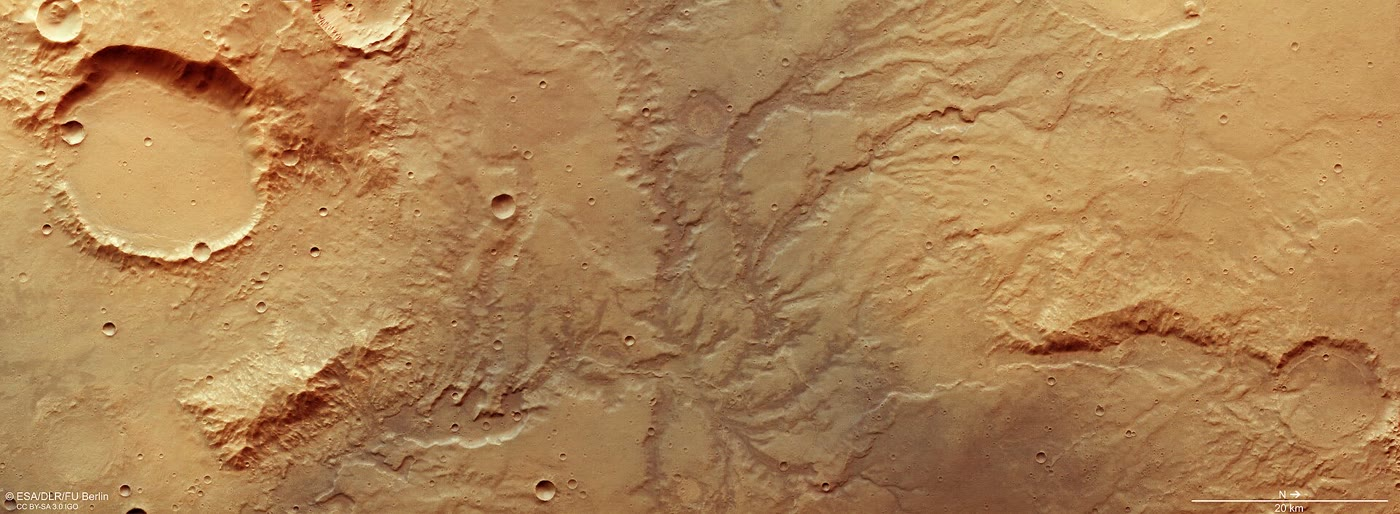
\includegraphics[width=\linewidth]{images/book5/b3-mars-valley-network.jpg}
\par\smallskip{\small Jaringan lembah kering di Mars, terlihat oleh
kamera Mars Express pada sekitar \qty{14}{m} per piksel, dekat \ang{17}\,LS,
\ang{66}\,BT; utara berada di sebelah kanan, dan bilah skala adalah \qty{20}{km}.
Anak sungai bergabung di hilir menjadi lembah yang lebih besar, pola
dari jaringan drainase. Gambar ESA/DLR/FU Berlin, CC BY-SA 3.0 IGO.}\label{fig:b3:planetary-atmospheres:valleys}
\end{omfigure}
% ledger: photo:b3-mars-valley-network

Lembah dan alur aliran Mars memerlukan, menurut taksiran geologi,
lapisan air global dengan kedalaman 100 sampai \qty{1500}{m}, dibandingkan dengan 3 sampai
\qty{25}{m} dalam es dan udaranya masa kini. Sebagian besar sisanya lenyap ke angkasa.
Pengorbit MAVEN mengukur angin surya yang mengikis gas dari Mars sekitar
\qty{100}{g} per detik, tiga perempatnya terbawa ke ekor
di belakang planet, tempat angin surya mengalir, dan seperempatnya dalam pancaran
di atas kutub; selama
badai surya Maret 2015 kehilangan itu makin cepat, dan kemungkinan besar jauh
lebih cepat ketika Matahari muda lebih aktif. Mars juga kehilangan hidrogen, sekitar
\num{3e26} atom per detik rata-rata hari ini: jika berlangsung selama empat miliar
tahun, kehilangan itu setara dengan lapisan air global yang hanya sekitar \qty{4}{m} dalamnya.
% ledger: gilli25:h-loss, lasp:maven

Laju itu tidak selalu sama dengan laju hari ini. Kemiringan sumbu Mars, \ang{25.2}
sekarang, telah berayun antara 0 dan \ang{66} selama 250 juta tahun terakhir,
di sekitar rata-rata dekat \ang{35}, sedangkan kemiringan sumbu Bumi hanya berubah
lebih dari satu derajat. Gerakannya kacau dan tidak dapat dilacak mundur selama miliaran
tahun; kawah elips hasil tumbukan menyerempet, yang orientasinya
merekam kemiringan sumbu, menunjukkan rata-rata antara sekitar 10 dan \ang{30} selama
sekitar 3.5 miliar tahun terakhir. Pada kemiringan tinggi, kutub musim panas menghangat,
lebih banyak uap air naik, dan model iklim membuat kehilangan hidrogen
dua puluh kali lebih cepat: sepanjang sejarah Mars, kehilangan itu setara dengan lapisan
sekitar \qty{80}{m}.
% ledger: planet:Mars.obliq, gilli25:obliquity, holo18:obliquity, gilli25:h-loss

\section{Titan: siklus metana}\label{sec:b3:planetary-atmospheres:titan}

Titan, sebuah bulan yang lebih kecil daripada Mars, memiliki atmosfer yang lebih tebal daripada Bumi:
tekanan permukaannya sekitar 60\,\% lebih tinggi, pada \qty{-179}{\degreeCelsius}.
Atmosfernya sekitar 95\,\% nitrogen dan 5\,\% metana, dan karena
gravitasi bulan ini lemah, atmosfernya membentang sepuluh kali lebih tinggi daripada Bumi, hingga
hampir \qty{600}{km}. Sinar ultraviolet memecah metana dan nitrogen
di lapisan atas; pecahannya bergabung kembali menjadi kabut jingga dari hidrokarbon yang lebih berat
yang menyembunyikan permukaan dari cahaya tampak. Di bawah kabut,
metana berperan seperti air: ia mengembun menjadi awan, turun sebagai hujan, memotong
alur sungai, serta mengisi danau dan laut metana dan etana.
% ledger: nasa:titan-surface, nasa:titan-facts

\begin{omfigure}
\centering
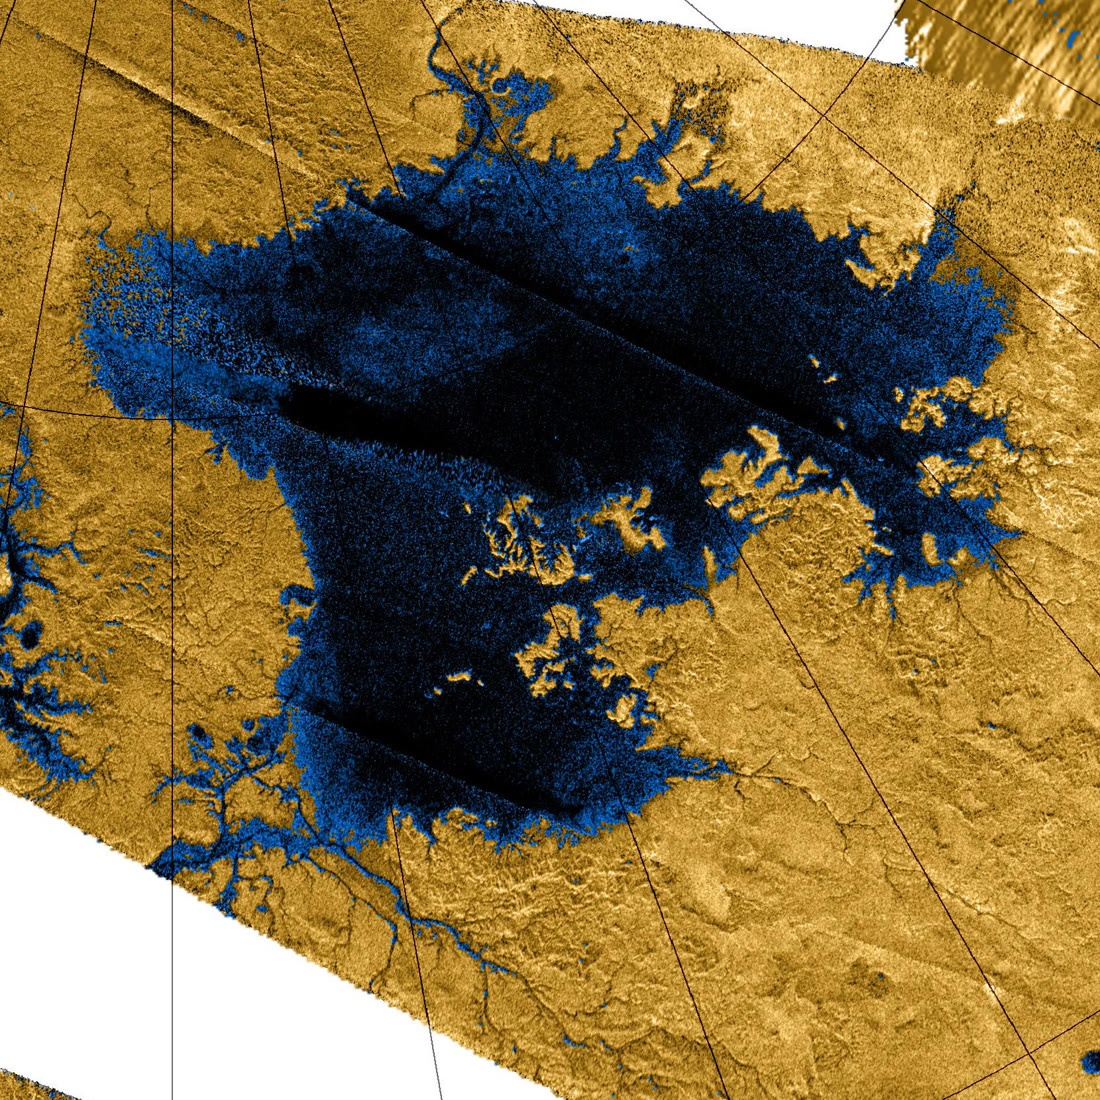
\includegraphics[width=0.5\linewidth]{images/book5/b3-ligeia-mare.jpg}
\par\smallskip{\small Ligeia Mare, sebuah laut dekat Kutub Utara Titan, dalam
mosaik warna semu citra radar Cassini: fitur yang diduga
cair berwarna biru dan hitam, daratan padat berwarna cokelat, dengan teluk, pulau
dan jaringan anak sungai yang diperkirakan. Dari sekitar 400 danau dan laut di
belahan utara yang terpetakan, yang lebih besar dari \qty{26000}{km^2} menampung 70\,\% luasnya.
NASA/JPL/USGS, domain publik.}\label{fig:b3:planetary-atmospheres:ligeia}
\end{omfigure}
% ledger: photo:b3-ligeia-mare

Apakah sebuah cairan dapat berada di permukaan bergantung pada diagram fasenya dan pada
tekanan serta suhu di sana. Permukaan Titan berada tepat di atas
titik tripel metana, \qty{90.67}{K} dan \qty{0.117}{bar}, dan di bawah
titik kritisnya: metana cair mungkin ada, dan metana pada 5\,\% dari
\qty{1.6}{bar} tidak jauh dari kejenuhan. Permukaan Mars berada dekat
titik tripel air, sedangkan Bumi berada jauh di dalam daerah cairnya, dan
Venus berada di atas suhu kritis air, \qty{647}{K}, tempat tidak ada
cairan yang dapat ada sama sekali.
% ledger: nist:methane-phase, iapws:triple-critical, nasa:titan-surface

\begin{omfigure}
\centering
\begin{tikzpicture}
\begin{axis}[width=0.8\linewidth, height=0.52\linewidth,
  xmin=60, xmax=800, ymin=1e-4, ymax=1000, ymode=log,
  xlabel={suhu (\unit{K})}, ylabel={tekanan (\unit{bar})},
  tick label style={font=\scriptsize}, label style={font=\small}]
\addplot[thick, omDef] table[x=T, y=p_bar] {figdata/out/bachelor-3-habitability-water.dat};
\addplot[thick, omDef, dashed] table[x=T, y=p_bar] {figdata/out/bachelor-3-habitability-ice.dat};
\addplot[thick, orange!80!black] table[x=T, y=p_bar] {figdata/out/bachelor-3-habitability-methane.dat};
\addplot[only marks, mark=*, mark size=1.6pt, omDef] coordinates {(273.16,0.00611657) (647.096,220.64)};
\addplot[only marks, mark=*, mark size=1.6pt, orange!80!black] coordinates {(90.67,0.1169) (190.6,46.1)};
\addplot[only marks, mark=square*, mark size=2.2pt, black] table[x=T, y=p_bar] {figdata/out/bachelor-3-habitability-bodies.dat};
\node[font=\scriptsize, anchor=south] at (axis cs:737,110) {Venus};
\node[font=\scriptsize, anchor=west] at (axis cs:300,1.0) {Bumi};
\node[font=\scriptsize, anchor=north] at (axis cs:214,0.0045) {Mars};
\node[font=\scriptsize, anchor=south] at (axis cs:94,2.2) {Titan};
\node[font=\scriptsize, omDef, anchor=west] at (axis cs:420,3) {air: cair di atas, uap di bawah};
\node[font=\scriptsize, omDef, anchor=north west] at (axis cs:205,0.0012) {es};
\node[font=\scriptsize, orange!80!black, anchor=west] at (axis cs:196,46) {metana};
\node[font=\scriptsize, omDef, anchor=south east] at (axis cs:640,230) {titik kritis};
\end{axis}
\end{tikzpicture}
\par\smallskip{\small Batas antara uap dan air yang terkondensasi
(biru: cair--uap, dari titik tripel ke titik kritis;
putus-putus: es--uap) dan antara metana cair dan uapnya (oranye),
dengan keadaan permukaan rata-rata Venus, Bumi, Mars, dan Titan
(kotak). Cairan dapat berada di permukaan yang tekanannya di atas
kurva cairan itu, di antara suhu tripelnya dan
suhu kritisnya.}\label{fig:b3:planetary-atmospheres:phases}
\end{omfigure}
% ledger: iapws:vapour-pressure, iapws4:sublimation, iapws:triple-critical, nist:methane-phase, nasa:venus-atm, planet:Earth.Tmean, planet:Earth.psurf, nasa:mars-atm, nasa:titan-surface

Titan mempertahankan nitrogennya dengan mudah: pada \omterm{def:b3:planetary-atmospheres:exobase}{eksobasenya} $\lambda = 41$ untuk
nitrogen. Hidrogennya, dengan $\lambda$ sekitar 1.5, lolos hampir bebas, dan
lolos hidrogen molekuler ditentukan lebih rendah oleh fluks pembatas
melalui \omterm{def:b3:planetary-atmospheres:hydrodynamic}{homopause}, seperti di Bumi. Senyawa berat yang terbentuk dari
metana yang pecah mengendap ke permukaan, tempat ia membentuk pasir hamparan
gumuk pasir yang luas.
% ledger: gronoff:jeans-table, gronoff:diffusion, nasa:titan-surface

\section{Kelayakhunian planet}\label{sec:b3:planetary-atmospheres:habitability}

Zona layak huni buku sekolah adalah rentang jarak dari sebuah bintang
tempat planet seperti Bumi dapat mempertahankan air cair di
permukaannya. Tepinya adalah batas-batas yang ditemui dalam bab ini.

\begin{definition}[Kelayakhunian planet]\label{def:b3:planetary-atmospheres:habitability}
Yang disebut \emph{kelayakhunian planet}\index{kelayakhunian planet} sebuah
planet adalah kemampuannya mempertahankan air cair di permukaannya selama
waktu geologi: ia menerima fluks bintang dalam batas
zona layak huni, ia menahan atmosfer dan airnya agar tidak
lolos, dan siklus karbon jangka panjang mengatur iklimnya.
\end{definition}

Tepi dalam zona layak huni adalah \omterm{def:b3:planetary-atmospheres:runaway}{rumah kaca lembap} atau
\omterm{def:b3:planetary-atmospheres:runaway}{rumah kaca tak terkendali}: planet mirip Bumi di sekitar Matahari menjadi lembap pada
\qty{0.99}{au} dan menjadi tak terkendali pada \qty{0.97}{au}. Tepi luarnya adalah
\emph{rumah kaca maksimum}: menambah karbon dioksida hanya memanaskan planet sampai
gas tambahan memantulkan lebih banyak sinar Matahari daripada efek rumah kacanya;
yang diperolehnya; di sekitar Matahari hal ini terjadi pada
\qty{1.70}{au}, pada sekitar \qty{8}{bar} karbon dioksida. Itu adalah
tepi konservatif, dihitung tanpa awan. Dua tepi empiris lebih lebar:
Venus tampaknya tidak memiliki air permukaan selama setidaknya satu miliar tahun,
ketika ia menerima 1.76 kali sinar Matahari Bumi saat ini (\qty{0.75}{au});
Mars memiliki air mengalir ketika ia menerima 0.32 kali sinar tersebut, jika lembahnya
berumur 3.8 miliar tahun (\qty{1.77}{au}). Di sekitar bintang yang lebih dingin, batas yang sama tercapai
pada fluks yang lebih rendah, karena cahayanya yang lebih merah kurang terhambur dan
lebih banyak diserap oleh air dan karbon dioksida.
% ledger: kopparapu13:runaway, kopparapu13:outer, kopparapu13:hz-fit

\begin{omfigure}
\centering
\begin{tikzpicture}
\begin{axis}[width=0.8\linewidth, height=0.5\linewidth,
  xmin=0, xmax=2.1, ymin=2600, ymax=7200, x dir=reverse,
  xlabel={fluks bintang yang diterima / Bumi saat ini},
  ylabel={suhu bintang (\unit{K})},
  tick label style={font=\scriptsize}, label style={font=\small},
  legend style={font=\scriptsize, at={(0.5,-0.24)}, anchor=north, legend columns=2, draw=none}]
\addplot[name path=mg, thick, omDef] table[x=mg, y=Teff] {figdata/out/bachelor-3-habitability-hz.dat};
\addlegendentry{rumah kaca lembap}
\addplot[name path=maxg, thick, red!70!black] table[x=maxg, y=Teff] {figdata/out/bachelor-3-habitability-hz.dat};
\addlegendentry{rumah kaca maksimum}
\addplot[thin, omDef, dashed] table[x=rg, y=Teff] {figdata/out/bachelor-3-habitability-hz.dat};
\addlegendentry{rumah kaca tak terkendali}
\addplot[thin, black!60, densely dotted] table[x=rv, y=Teff] {figdata/out/bachelor-3-habitability-hz.dat};
\addlegendentry{Venus masa kini, Mars awal}
\addplot[thin, black!60, densely dotted, forget plot] table[x=em, y=Teff] {figdata/out/bachelor-3-habitability-hz.dat};
\addplot[green!30, opacity=0.5, forget plot] fill between[of=mg and maxg];
\addplot[only marks, mark=*, mark size=2pt, black, forget plot] coordinates {(1.911,5780) (1.0,5780) (0.431,5780)};
\node[font=\scriptsize, anchor=south] at (axis cs:1.911,5800) {Venus};
\node[font=\scriptsize, anchor=west, xshift=2pt] at (axis cs:1.0,5780) {Bumi};
\node[font=\scriptsize, anchor=east, xshift=-2pt] at (axis cs:0.431,5780) {Mars};
\end{axis}
\end{tikzpicture}
\par\smallskip{\small Zona layak huni planet mirip Bumi, sebagai
fluks bintang yang diterimanya terhadap suhu bintangnya (diarsir:
di antara \omterm{def:b3:planetary-atmospheres:runaway}{rumah kaca lembap} dan rumah kaca maksimum). Garis titik-titik: batas
empiris yang ditarik dari Venus masa kini dan Mars awal. Penyesuaian
tersebut berasal dari model iklim tanpa awan, berlaku dari 2600 hingga
\qty{7200}{K}.}\label{fig:b3:planetary-atmospheres:hz}
\end{omfigure}
% ledger: kopparapu13:hz-fit, nasa:venus, nasa:mars

Jarak saja tidak cukup. Planet harus mempertahankan atmosfernya: planet yang kecil
atau panas, yang \omterm{def:b3:planetary-atmospheres:jeans-escape}{parameter lolosnya} rendah, kehilangan hidrogennya dan bersamanya
airnya, dan planet di dalam \omterm{def:b3:planetary-atmospheres:runaway}{rumah kaca lembap} mengering dari atas. Ia
juga harus menjaga iklimnya tetap stabil selama miliaran tahun sementara bintangnya
makin terang: di Bumi, termostat pelapukan silikat dari
siklus karbon jangka panjang menarik turun karbon dioksida saat iklim menghangat
dan membiarkannya menumpuk saat iklim mendingin. Di Venus, tanpa tektonik lempeng,
karbon dioksida yang keluar dari dalam planet tidak punya jalan kembali ke batuan dan
menumpuk di udara; kini ia menyimpan kira-kira sebanyak karbon dioksida yang
Bumi terkunci dalam batuan karbonat. Apakah medan magnet melindungi
atmosfer masih diperdebatkan: medan itu melindungi atmosfer atas dari angin
Matahari, tetapi juga membuka jalur lolos lain, seperti aliran keluar ion
di dekat kutub, dan \omterm{def:b3:planetary-atmospheres:habitability}{kelayakhunian planet} tidak dapat dibaca dari
posisinya dalam zona layak huni saja.
% ledger: arney18:venus-loss, gronoff21:magnetic, gronoff:nonthermal

\section{Latihan}

\begin{exercise}[$\star$]\label{exo:b3:planetary-atmospheres:1}
Hitung tinggi skala $H = RT/Mg$ dekat permukaan Venus
(\qty{737}{K}, karbon dioksida dengan massa molar \qty{44.01}{g.mol^{-1}},
$g = \qty{8.87}{m.s^{-2}}$), Bumi (\qty{288}{K},
\qty{28.97}{g.mol^{-1}}, \qty{9.80}{m.s^{-2}}), Mars (\qty{214}{K},
\qty{43.34}{g.mol^{-1}}, \qty{3.71}{m.s^{-2}}) dan Titan (\qty{94}{K},
\qty{28.0}{g.mol^{-1}}, \qty{1.35}{m.s^{-2}}). Atmosfer mana yang paling
mengembang, dan mengapa?
\end{exercise}

\begin{exercise}[$\star$]\label{exo:b3:planetary-atmospheres:2}
\omterm{def:b3:planetary-atmospheres:exobase}{Eksobase} Bumi berada pada \qty{500}{km} (jari-jari \qty{6878}{km});
suhunya bervariasi dari 800 hingga \qty{1600}{K} sepanjang siklus Matahari.
Ambil massa Bumi sebagai \qty{5.97e24}{kg}. Hitung \omterm{def:b3:planetary-atmospheres:jeans-escape}{parameter lolos}
atom hidrogen pada kedua suhu itu, dan fraksi yang lolos
$(1 + \lambda)e^{-\lambda}$. Dengan faktor berapa siklus Matahari mengubahnya?
\end{exercise}

\begin{exercise}[$\star$]\label{exo:b3:planetary-atmospheres:3}
Di sekitar Matahari, planet mirip Bumi berubah menjadi lembap pada fluks $S_\mathrm{eff}
= 1.014$, masuk \omterm{def:b3:planetary-atmospheres:runaway}{rumah kaca tak terkendali} pada 1.0512 dan mencapai rumah kaca maksimum pada 0.3438
(fluks relatif terhadap Bumi). (a)~Hitung ketiga jarak, dalam
satuan astronomi. (b)~Venus dan Mars menerima 1.91 dan 0.43 kali
sinar Matahari yang diterima Bumi. Tentukan posisi keduanya.
\end{exercise}

\begin{exercise}[$\star$]\label{exo:b3:planetary-atmospheres:4}
Tekanan uap metana cair adalah $\log_{10}(p/\unit{bar}) = 3.9895 -
443.028/(T/\unit{K} - 0.49)$. (a)~Hitung tekanan uap itu di permukaan Titan,
\qty{94.15}{K}. (b)~Metana menyusun 5\,\% udara Titan pada \qty{1.6}{bar}.
Hitung tekanan parsialnya dan kelembapan relatifnya. (c)~Apa yang
disarankan hasil itu tentang penguapan dari laut Titan?
\end{exercise}

\begin{exercise}[$\star\star$]\label{exo:b3:planetary-atmospheres:5}
Pada \omterm{def:b3:planetary-atmospheres:exobase}{eksobase} Bumi (\qty{1000}{K}, $\lambda = 7.02$ untuk hidrogen),
hitung \omterm{def:b3:planetary-atmospheres:jeans-escape}{parameter lolos} deuterium, kecepatan termalnya relatif terhadap
hidrogen, dan rasio fluks Jeans per atom, D terhadap H. Apakah \omterm{def:b3:planetary-atmospheres:jeans-escape}{lolos Jeans}
bertindak sebagai saringan isotop yang kuat?
\end{exercise}

\begin{exercise}[$\star\star$]\label{exo:b3:planetary-atmospheres:6}
Rasio D/H air Venus adalah \num{0.016}; air samudra di
Bumi adalah \num{1.5575e-4}. (a)~Hitung pengayaannya. (b)~Tanpa
lolosnya deuterium sama sekali, berapa jumlah air Venus terkecil di masa lalu,
bila hari ini \qty{6e15}{kg}? Berapa kedalaman yang terbentuk jika tersebar di
permukaan planet seluas \qty{4.60e14}{m^2}? (c)~Berapa penyusutan cadangan
yang dibutuhkan \omterm{def:b3:planetary-atmospheres:hydrodynamic}{lolos terbatas-difusi} dengan $\alpha = 0.8$? Simpulkan.
\end{exercise}

\begin{exercise}[$\star\star$]\label{exo:b3:planetary-atmospheres:7}
Mars, dengan jari-jari \qty{3389.5}{km}, kehilangan sekitar \num{3e26} atom hidrogen
per detik. (a)~Jika setiap pasang atom berasal dari satu molekul air, seberapa
tebal lapisan air global yang dihilangkan oleh kehilangan itu dalam empat miliar tahun?
(b)~Pertanyaan yang sama pada \num{6e27} atom per detik, laju pada
obliquitas tinggi. (c)~Bandingkan dengan 100 hingga \qty{1500}{m} yang dibutuhkan
lembah dan alur.
\end{exercise}

\begin{exercise}[$\star\star$]\label{exo:b3:planetary-atmospheres:8}
(a)~Hitung massa atmosfer Mars dari tekanan permukaan rata-rata,
\qty{636}{Pa}, gravitasinya, \qty{3.71}{m.s^{-2}}, dan jari-jarinya.
(b)~Angin matahari mengikis sekitar \qty{100}{g} gas per detik.
Berapa massa yang hilang dalam empat miliar tahun, dan dalam berapa lama ia akan menghilangkan atmosfer sekarang?
(c)~Mengapa itu merupakan taksiran yang terlalu rendah untuk
kehilangan di masa lalu?
\end{exercise}

\begin{exercise}[$\star\star$]\label{exo:b3:planetary-atmospheres:9}
Planet mirip Bumi dengan atmosfer uap tanpa awan memantulkan 19.3\,\%
dari cahaya matahari yang diterimanya; keluaran inframerahnya tidak boleh melebihi
\qty{291}{W.m^{-2}}. (a)~Di atas fluks cahaya matahari berapa, dalam watt per
meter persegi dan relatif terhadap \qty{1361}{W.m^{-2}} Bumi, ia mengalami \omterm{def:b3:planetary-atmospheres:runaway}{rumah kaca tak terkendali}?
(b)~Bandingkan dengan Venus masa kini, \qty{2601}{W.m^{-2}}, dan dengan Venus muda
di bawah Matahari yang luminositasnya 70\,\% dari luminositas sekarang. (c)~Mengapa
kesimpulan untuk Venus muda belum final?
\end{exercise}

\begin{exercise}[$\star\star\star$]\label{exo:b3:planetary-atmospheres:10}
Model termosfer oksigen atomik bersifat isotermal pada \qty{1000}{K}, dengan
$n = \qty{1e16}{m^{-3}}$ pada \qty{200}{km}; ambil $g =
\qty{9.21}{m.s^{-2}}$ pada ketinggian itu dan penampang lintang tumbukan
$\sigma_c = \qty{3e-19}{m^2}$. (a)~Hitung tinggi skala oksigen.
(b)~Hitung massa jenis pada \omterm{def:b3:planetary-atmospheres:exobase}{eksobase} dan tinggi \omterm{def:b3:planetary-atmospheres:exobase}{eksobase}.
(c)~Gravitasi berkurang dengan ketinggian. Apakah itu menggeser \omterm{def:b3:planetary-atmospheres:exobase}{eksobase} ke atas atau
ke bawah?
\end{exercise}

\begin{exercise}[$\star\star\star$]\label{exo:b3:planetary-atmospheres:11}
(a)~Misalkan stratosfer Bumi menjadi lembap, dengan rasio campuran
uap air sebesar \num{3e-3} (dihitung sebagai $\ce{H2}$). Dengan batas difusi
$\num{3.0e13}\,f$ molekul $\ce{H2}$ per sentimeter persegi dan
per detik, pada \qty{200}{K}, hitung kehilangan hidrogen dari seluruh
Bumi (jari-jari \qty{6371}{km}). (b)~Berapa lama samudra,
\qty{1.4e24}{g} air, akan bertahan? Bandingkan dengan umur Bumi.
\end{exercise}

\begin{exercise}[$\star\star\star$]\label{exo:b3:planetary-atmospheres:12}
Dalam atmosfer atas uap murni yang menyerap sebagai gas kelabu dengan $\kappa =
\qty{0.005}{m^2.kg^{-1}}$, pada planet dengan $g = \qty{9.81}{m.s^{-2}}$
dan $D = 1.66$: (a)~hitung tekanan $p_1$ pada aras pemancar;
(b)~dengan $p_\mathrm{sat}(T) = \qty{611.657}{Pa}\,\exp[(L/R_v)(1/T_t -
1/T)]$, $L = \qty{2.5e6}{J.kg^{-1}}$, $R_v = \qty{461.5}{J.kg^{-1}.K^{-1}}$,
$T_t = \qty{273.16}{K}$, hitung suhunya dan batas radiasinya.
(c)~Batas garis-demi-garis adalah \qty{291}{W.m^{-2}}. Haruskah
$\kappa$ efektif uap air sungguhan lebih besar atau lebih kecil?
\end{exercise}

\section{Soal: Akankah Kepos mempertahankan airnya?}

\begin{problem}[{Soal akhir pekan --- lolos dan kelayakhunian planet
samudra rekaan}]
\label{pb:b3:planetary-atmospheres:1}
Kepos adalah planet rekaan bermassa \qty{5.2e24}{kg} dan berjari-jari
\qty{6200}{km}, dengan samudra dan atmosfer nitrogen serta karbon
dioksida. Planet ini mengorbit pada \qty{0.60}{au} sebuah bintang dengan luminositas 0.30 kali
Matahari dan suhu efektif \qty{4800}{K}. \omterm{def:b3:planetary-atmospheres:exobase}{Eksobasenya} terletak
\qty{500}{km} di atas permukaan, pada \qty{1400}{K}, dengan
\qty{2e11}{m^{-3}} atom hidrogen; \omterm{def:b3:planetary-atmospheres:hydrodynamic}{homopausenya} berada pada \qty{200}{K},
tempat karbon dioksida mendominasi dan tempat hidrogen dalam segala bentuknya membentuk
rasio campuran $f = \num{1e-3}$, dihitung sebagai $\ce{H2}$. Samudra Bumi adalah
\qty{1.4e24}{g} air.

\medskip\noindent\textbf{Bagian I --- Eksobase.}
\begin{enumerate}
\item Hitung gravitasi permukaan dan massa jenis rata-rata Kepos.
\item Hitung kecepatan lepas pada \omterm{def:b3:planetary-atmospheres:exobase}{eksobase}.
\item Hitung kecepatan termal $u = \sqrt{2kT/m}$ hidrogen, helium, dan
  atom oksigen pada \omterm{def:b3:planetary-atmospheres:exobase}{eksobase}.
\item Hitung \omterm{def:b3:planetary-atmospheres:jeans-escape}{parameter lolos} mereka.
\item Yang manakah dari mereka yang dapat lolos melalui \omterm{def:b3:planetary-atmospheres:jeans-escape}{lolos Jeans} dengan laju berarti?
  Apakah ada yang mendekati rezim hidrodinamik?
\item Selama masa muda aktif bintangnya, \omterm{def:b3:planetary-atmospheres:exobase}{eksobase} Kepos mungkin pernah
  mencapai \qty{3000}{K}. Berapakah \omterm{def:b3:planetary-atmospheres:jeans-escape}{parameter lolos} hidrogen saat itu,
  dan apa yang disarankannya?
\end{enumerate}

\medskip\noindent\textbf{Bagian II --- Lolos Jeans pada hidrogen.}
\begin{enumerate}[resume]
\item Hitung fraksi yang lolos $(1 + \lambda)e^{-\lambda}$ untuk
  hidrogen.
\item Hitung fluks Jeans hidrogen, per meter persegi dan per detik.
\item Hitung jumlah atom hidrogen yang meninggalkan seluruh \omterm{def:b3:planetary-atmospheres:exobase}{eksobase}
  per detik.
\item Berapa banyak atom hidrogen yang dikandung samudra Bumi?
\item Dengan laju ini, berapa lama Kepos akan kehilangannya?
\item Hitung \omterm{def:b3:planetary-atmospheres:jeans-escape}{parameter lolos} deuterium dan efisiensi lolosnya
  relatif terhadap hidrogen, per atom.
\end{enumerate}

\medskip\noindent\textbf{Bagian III --- Batas difusi.}
\begin{enumerate}[resume]
\item Hitung tinggi skala karbon dioksida pada \omterm{def:b3:planetary-atmospheres:hydrodynamic}{homopause}.
\item Parameter difusi biner hidrogen dalam karbon dioksida adalah
  $b = \qty{1.2e19}{cm^{-1}.s^{-1}}$ pada \qty{200}{K}. Hitung
  fluks $\ce{H2}$ terbatas-difusi, per meter persegi dan per detik.
\item Periksa terhadap batas Bumi, $\num{3.0e13}\,f$ molekul per
  sentimeter persegi dan per detik, yang diskalakan dengan gravitasi.
\item Hitung jumlah atom hidrogen yang dapat dipasok batas difusi
  ke atmosfer atas seluruh planet per detik (ambil
  luas permukaannya).
\item Bandingkan dengan pertanyaan~9. Proses apa yang membatasi lolos, dan apa
  yang terjadi pada hidrogen termosfer?
\item Berapa kerapatan hidrogen pada \omterm{def:b3:planetary-atmospheres:exobase}{eksobase} yang memungkinkan \omterm{def:b3:planetary-atmospheres:jeans-escape}{lolos Jeans} membawa
  seluruh pasokan?
\item Berapa lama Kepos akan kehilangan samudra Bumi berupa hidrogen pada
  laju terbatas-difusi?
\end{enumerate}

\medskip\noindent\textbf{Bagian IV --- Apakah Kepos berada di zona layak huni?}
\begin{enumerate}[resume]
\item Hitung fluks bintang yang diterima Kepos, relatif terhadap Bumi.
\item Untuk bintang \qty{4800}{K}, batas \omterm{def:b3:planetary-atmospheres:runaway}{rumah kaca lembap} berada pada
  $S_\mathrm{eff} = 0.939$ dan rumah kaca maksimum pada 0.290. Hitung
  tepi zona layak huni, dalam satuan astronomi, dan tempatkan Kepos.
\item Dengan faktor berapa bintang harus menjadi lebih terang sebelum Kepos mencapai
  tepi dalam?
\item Dengan albedo 0.3, hitung cahaya matahari yang diserap Kepos per meter
  persegi, dan suhu kesetimbangannya. Bandingkan dengan \omterm{def:b3:planetary-atmospheres:runaway}{batas
  rumah kaca tak terkendali}.
\item Jika iklim yang lebih hangat membuat stratosfer Kepos lembap, dengan
  $f = \num{3e-3}$, berapa lama samudra Bumi akan bertahan?
\item Berikan waktu bagi Kepos untuk kehilangan samudra Bumi berupa hidrogen melalui
  \omterm{def:b3:planetary-atmospheres:hydrodynamic}{lolos terbatas-difusi} dengan $f = \num{1e-3}$, dalam miliar tahun, hingga
  dua angka signifikan.
\end{enumerate}
\end{problem}
% ledger: zahnle19:diffusion, kopparapu13:hz-fit, kopparapu13:runaway, gronoff:jeans, const:G, const:kB, const:NA
